% !TEX root = ../../prj4projektdokumentation.tex

\section{Brugergrænseflade}
\label{HMI}

Brugergrænsefladen består i dette projekt af en HMI KTP 600. Denne sidder på samme board som PLC'en og kan tilgåes gennem swicthen !!!!CSM!!!. Den har to skærme; automatisk og manuel mode, hvoraf automatisk mode er startskærm ved opstart.


Det skal nævnes at systemet først var tiltænkt at have tre Måleenheder, så derfor er det klargjort til tre, men kun de to er brugt i systemet, da det vigtigste er proof of concept. Felterne under Måleenhed forbruger 2 er derfor ikke aktive.

\subsection{Automatisk mode}

Formålet med HMI'et var at en bruger skulle kunne observere målinger fra Måleenhederne og følge med i hvilket trin transformer brugte. I automatisk mode, som er vist på figur \ref{fig:HMIAutomatiskModeDesign}, skal en bruger ikke kunne interagere med systemet udover at kunne skifte til manuel mode.
Generelt var tanken det skulle være overskueligt for brugeren, derfor er måleværdier og placering opsat som rækker og kolonner. Alt der har med trinskifteren at gøre er blevet placeret nederst, under en skillelinje for at give overblik for brugeren.

\begin{figure}[H] % (alternativt [H])
	\centering
	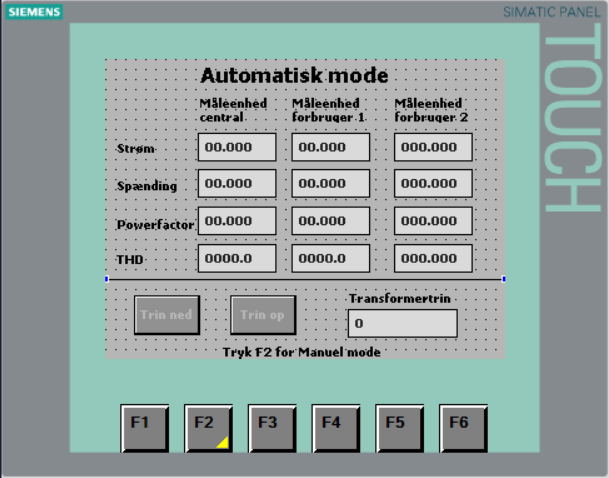
\includegraphics[width=0.7\textwidth]{Figure/HMIAutomatiskModeDesign}
	\caption{Screenshot af HMI i automatisk mode}
	\label{fig:HMIAutomatiskModeDesign}
\end{figure}

For at skifte til manuel mode trykkes på knappen F2, for at det er tydeligt at et tryk ville indebære en stor ændring i programmet. Det er også skrevet på selve skærmen for at gøre en bruger opmærksom på tilstandsskiftet. Måden skiftet er programmeret er gennem eventet Press Key og funktionen ActivateScreen, som kan ses på figur \ref{fig:ActivateScreen}.

\begin{figure}[H] % (alternativt [H])
	\centering
	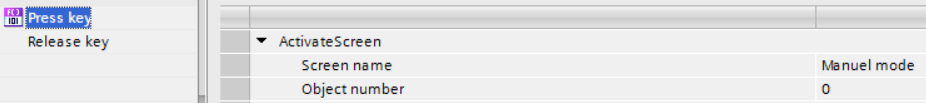
\includegraphics[width=0.8\textwidth]{Figure/ActivateScreen}
	\caption{Aktiver manuel mode skærmen}
	\label{fig:ActivateScreen}
\end{figure}

Måleværdierne er koblet med de word arrays DataCentralEnhed og DataDecentralEnhed tidligere omtalt i afsnit !!!!REF TIL DEM!!!. Dette sker gennnem opsætning af Inoutblokkene. Et eksempel kan ses på figur \ref{fig:OutputblokMaelingStroemCentral} for strømmen ved den centrale måleenhed, hvor det tilknyttede PLC tag er DataCentralEnhed[0]. Plads 0 er altid strømmen, ligegyldigt hvilket array der tales om. Plads 1 er spændingen, plads 2 er powerfactor og plads 3 er THD. Blokken er sat til mode output, dvs. at man ikke kan ændre værdien gennem skærmen. Formatet er et decimaltal med to decimaler før punktummet og tre decimaler efter punktummet.
Værdien blokkene er tilknyttet er for strøm og spænding i milliammpere og millivolt, derfor er kommaet flyttede tre pladser frem, så værdierne der vises er i ampere og volt.


Det forventes ikke at systemet under normale omstændigheder viser tal større end 7 volt, men to decimaler før kommaet er blevet valgt for at systemet kan vise selv meget store målinger, grundet fejl på distributionslinjen. Powerfactor er i transmissionen af data også blevet gjort 1000 gange større og derfor flyttes punktummet også tre pladser her. THD er før transmissionen et decimaltal, som er forstørret 1000 gange, så her er punktummet flyttet en plads for at det kan vises i procent for brugeren.

\begin{figure}[H] % (alternativt [H])
	\centering
	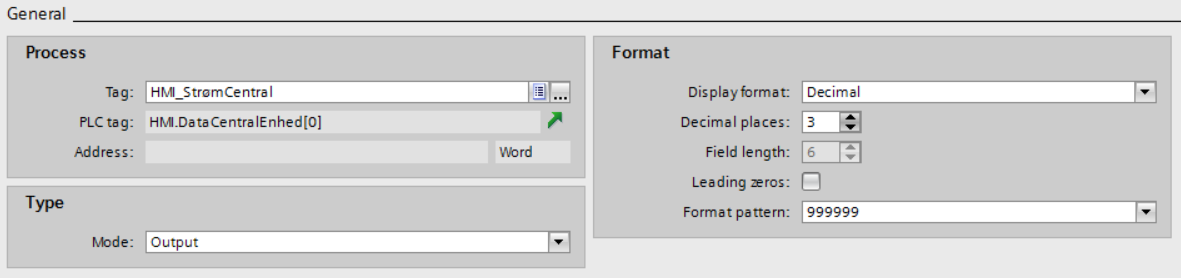
\includegraphics[width=1\textwidth]{Figure/OutputblokMaelingStroemCentral}
	\caption{Inoutblok for strømmåling ved central Måleenhed}
	\label{fig:OutputblokMaelingStroemCentral}
\end{figure}

Til visning af transformertrin er også valgt en Inoutblok, i mode Output og tilknyttet PLC tagget Trin brugt i FB'en Trinskifter. Trykknapperne Trin ned og Trin op er gråskalerede for at vise at de ikke er anvendelige i dette mode.

\subsection{Manuel mode}

Gennemgående er den samme model brugt til Manuel mode, men der er to forskelle. Den første er at for at skifte til automatisk mode skal bruges knappen F1, hvilket også er tydeliggjort ved en tekst nederst på skærmen.


Den anden er at knapperne Trin ned og Trin Op nu er aktive og kan bruges. Valget af sort tekst på hvid baggrund gør det nemt for en bruger at spotte at knapperne kan bruges. Figur \ref{fig:HMIManuelModeDesign} viser Manuel mode.

\begin{figure}[H] % (alternativt [H])
	\centering
	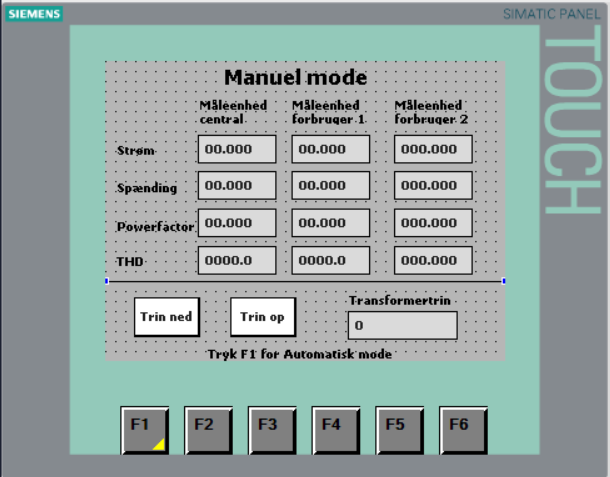
\includegraphics[width=0.5\textwidth]{Figure/HMIManuelModeDesign}
	\caption{Screenshot af HMI i manuel mode}
	\label{fig:HMIManuelModeDesign}
\end{figure}

Knappen er sat til at man ved et tryk sætter et bit, her er det tgget HMI\_KnapOp, der er tilknyttet PLC tagget KnapOp som anvendes i FB'en Trinskifter. Se figur \ref{fig:HMITrinOp}. Når knappen slippes er funktionen ResetBit anvendt, som resetter HMI\_KnapOp. Trin ned har samme funktionalitet, her er det bare HMI\_KnapNed, der anvendes, som er tilknyttet KnapNed i FB'en Trinskifter.

\begin{figure}[H] % (alternativt [H])
	\centering
	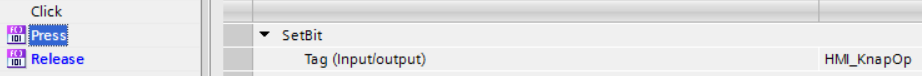
\includegraphics[width=0.8\textwidth]{Figure/HMITrinOp}
	\caption{Funktionalitet bag Trin op knappen}
	\label{fig:HMITrinOp}
\end{figure}

Ved tryk på knapperne F1 og F2 aktiveres skærmen for, henholdsvis automatisk og manuel mode, men dette sætter ikke programmet i de tilsvarende tilstand. Det sker i øjeblikket den pågældende skærm bliver loaded. Tilstanden styres af et bit der har HMI tagget HMI\_ManuelMode og PLC tagget ManuelMode. På figur \ref{fig:LoadManuelModeSkaerm} kan man se at når manuel mode skærmen loades kaldes SetBit funktionen. For automatisk mode skærmen kaldes funktionen ResetBit på samme bit.

\begin{figure}[H] % (alternativt [H])
	\centering
	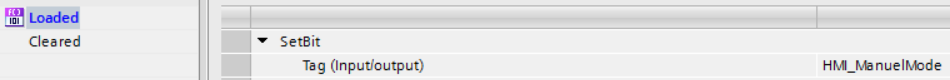
\includegraphics[width=0.8\textwidth]{Figure/LoadManuelModeSkaerm}
	\caption{Aktivering af manuel mode når manuel mode skærmen loades}
	\label{fig:LoadManuelModeSkaerm}
\end{figure}

Generalt er skærmene udviklet med henblik på at det er nemt få overblik over dem og at de er nemme at forstå. Der er valgt at ligge vægt på få muligheder, fordi det er et system som dette skal sikres mod forkert brug, da det kan få store konsekvenser.